% ----------------------------------------------------------
% APÊNDICE A - Algoritmos
% ----------------------------------------------------------
\begin{apendicesenv}
\chapter{Algoritmos}
\label{app:algoritmos}
	O algoritmo BinomialDistribution\_PROB tem como resultado a probabilidade de distribuição de um range e utiliza a fórmula  da probabilidade binomial geral abaixo. Esse algoritmo tem o mesmo resultado do algoritmo Distribution\_PROB, porém a execução do BinomialDistribution\_PROB é muito mais rápida e tem maior capacidade por usar números grandes como o BigInteger e o BigDecimal. Ambos os algoritmos foram feitos em C\# com o LINQPad 5 \footnotemark. Na Figura \ref{fig:BinomialDistribution_PROB_and_Distribution_PROB} é mostrado o resultado dos algoritmos para o range de 0 a 10, análogo ao lançamento de 10 moedas ao chão e somado os valores de caras e coras, sendo, por exemplo, a coroa com o valor um e a cara o valor dois. O algoritmo Distribution\_PROB soma cada uma das 1024 possibilidades [1,1,1,1,1,1,1,1,1,1 - 1,1,1,1,1,1,1,1,1,2 - ....] e agrupa esses valores somados. No algoritmo Distribution\_PROB esse conjunto de possibilidades é um produto cartesiano das possíveis combinações, o que torna esse algoritmo lento rapidamente, porém ele é importante para validar e facilitar o entendimento da a fórmula da probabilidade binomial geral utilizada no algoritmo BinomialDistribution\_PROB \cite{mathisfun_binomial_distribution}. Na Figura \ref{fig:BinomialDistribution_PROB_and_Distribution_PROB}, a tabela no interior de  Distribution\_PROB mostra esse agrupamento e o total de possibilidades, 1024. Ao dividir cada valor agrupado pelo total tem-se o resultado probabilístico alcançado pela fórmula empregada no BinomialDistribution\_PROB. Por exemplo, a probabilidade do somatório das 10 moedas lançadas ser 12 é igual a 45/1024, que é 0,0439453125 ou 4,39\%.
\footnotetext{O LINQPad 5 é encontrado em \url{www.linqpad.net} e pode ser utilizado em sua versão livre, Standard edition, sem expiração.}
\begin{align*}
f(k;n,p) &= \binom{n}{k} p^k(1 - p)^{n-k}
\end{align*}

\begin{figure}[H]
\caption{Resultado dos algoritmos  BinomialDistribution\_PROB e Distribution\_PROB}
\label{fig:BinomialDistribution_PROB_and_Distribution_PROB}
\centering
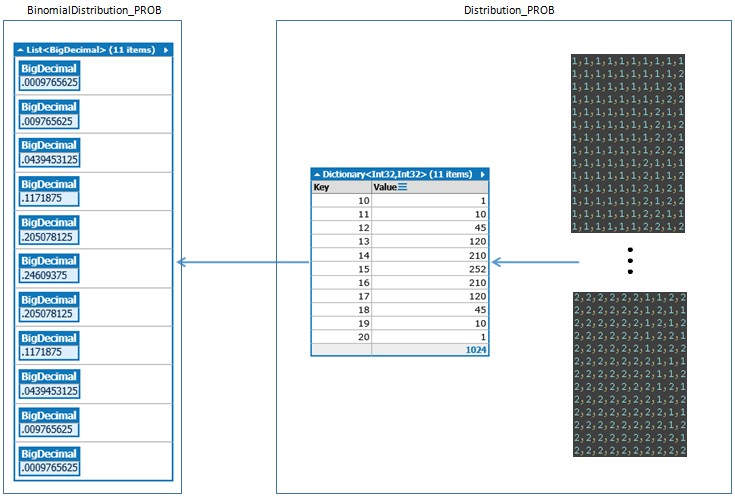
\includegraphics[scale=.75]{sections/images/BinomialDistribution_PROB_and_Distribution_PROB.jpg}
\floatfoot{O algoritmo Distribution\_PROB tem o intuito que clarificar a essência probabilística do teorema central do limite.} %\footnotemark.
\end{figure}

O algoritmo Distribution\_PROB também pode ser utilizado para o lançamento de 5 dados de 6 lados ou 6 dados de 5 lados, por exemplo. Como pode ser observado na Figura abaixo, a distribuição das probabilidades no lance dos dados é semelhante à distribuição binomial, das moedas.

\begin{figure}[H]
\centering
	\begin{subfigure}[H]{0.47\linewidth}
	\centering
	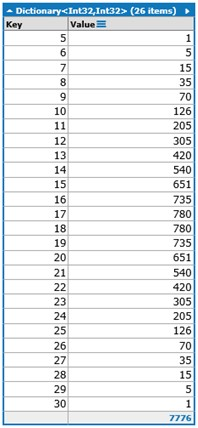
\includegraphics[width=.7\linewidth]{sections/images/Distribution_PROB_5_6.jpg}
	\caption{5 dados de 6 lados}
	\label{fig:Distribution_PROB_5_6}
	\end{subfigure}
\hfill
	\begin{subfigure}[H]{0.47\linewidth}
	\centering
	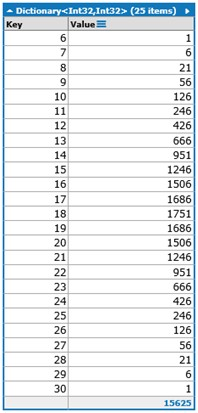
\includegraphics[width=.72\linewidth]{sections/images/Distribution_PROB_6_5.jpg}
	\caption{6 dados de 5 lados}
	\label{fig:Distribution_PROB_6_5}
	\end{subfigure}%
\caption{Resultados do algoritmo Distribution\_PROB}

\floatfoot{A distribuição das probabilidades no lance dos dados é consonante à distribuição binomial.} %\protect\footnotemark
\end{figure}

O algoritmo Logic\_WavePattern tem como resultado a exibição de um histograma que assume o padrão de ondas, quando colocados lado a lado cada uma de suas barras do lado esquerdo e lado direito da mediana. Esse histograma é gerado a partir da randomização de valores conforme Figura \ref{fig:consciousness_logical_moments} e Figura \ref{fig:consciousness}, seguindo o Teorema central do limite.

\begin{figure}[H]
\caption{Histograma em padrão de ondas do algoritmo Logic\_WavePattern}
\label{fig:logic_wavepattern_15000}
\centering
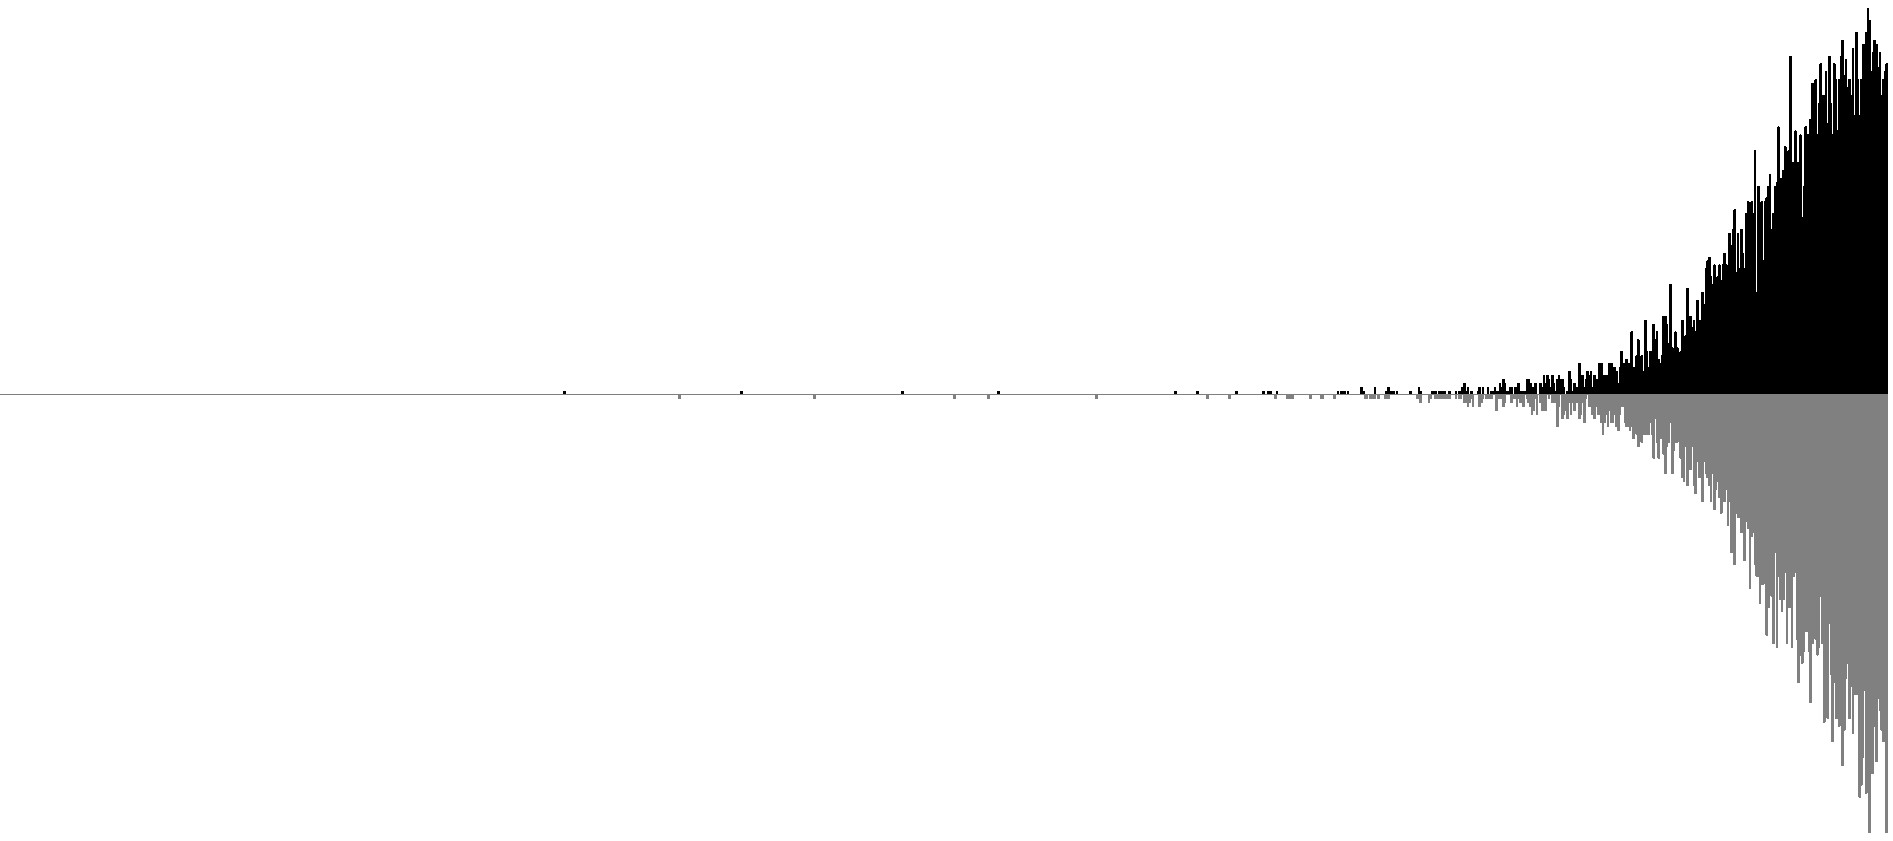
\includegraphics[scale=.25]{sections/images/logic_wavepattern_15000.jpg}
\floatfoot{Resultado gerado randomicamente e exibido pelo algoritmo Logic\_WavePattern.} %\footnotemark.
\end{figure}

Outro resultado do algoritmo Logic\_WavePattern é obtido a partir do console do LINQPad 5, onde se tem como saída um arquivo do tipo .csv que pode ser importado no Chart Studio da plotly \url{https://chart-studio.plot.ly/create} para geração de um gráfico de dispersão 3D. O mais importante do gráfico são os pontos que representam a matéria gerada a partir das ondas pelas três coordenadas do espaço, as linhas são usadas para facilitar a visualização das aspirais que já começam a se formar mesmo como volumes muito baixo de dados. 

\begin{figure}[H]
\caption{Gráfico de dispersão 3D do algoritmo Logic\_WavePattern}
\label{fig:plotly_3DScatter}
\centering
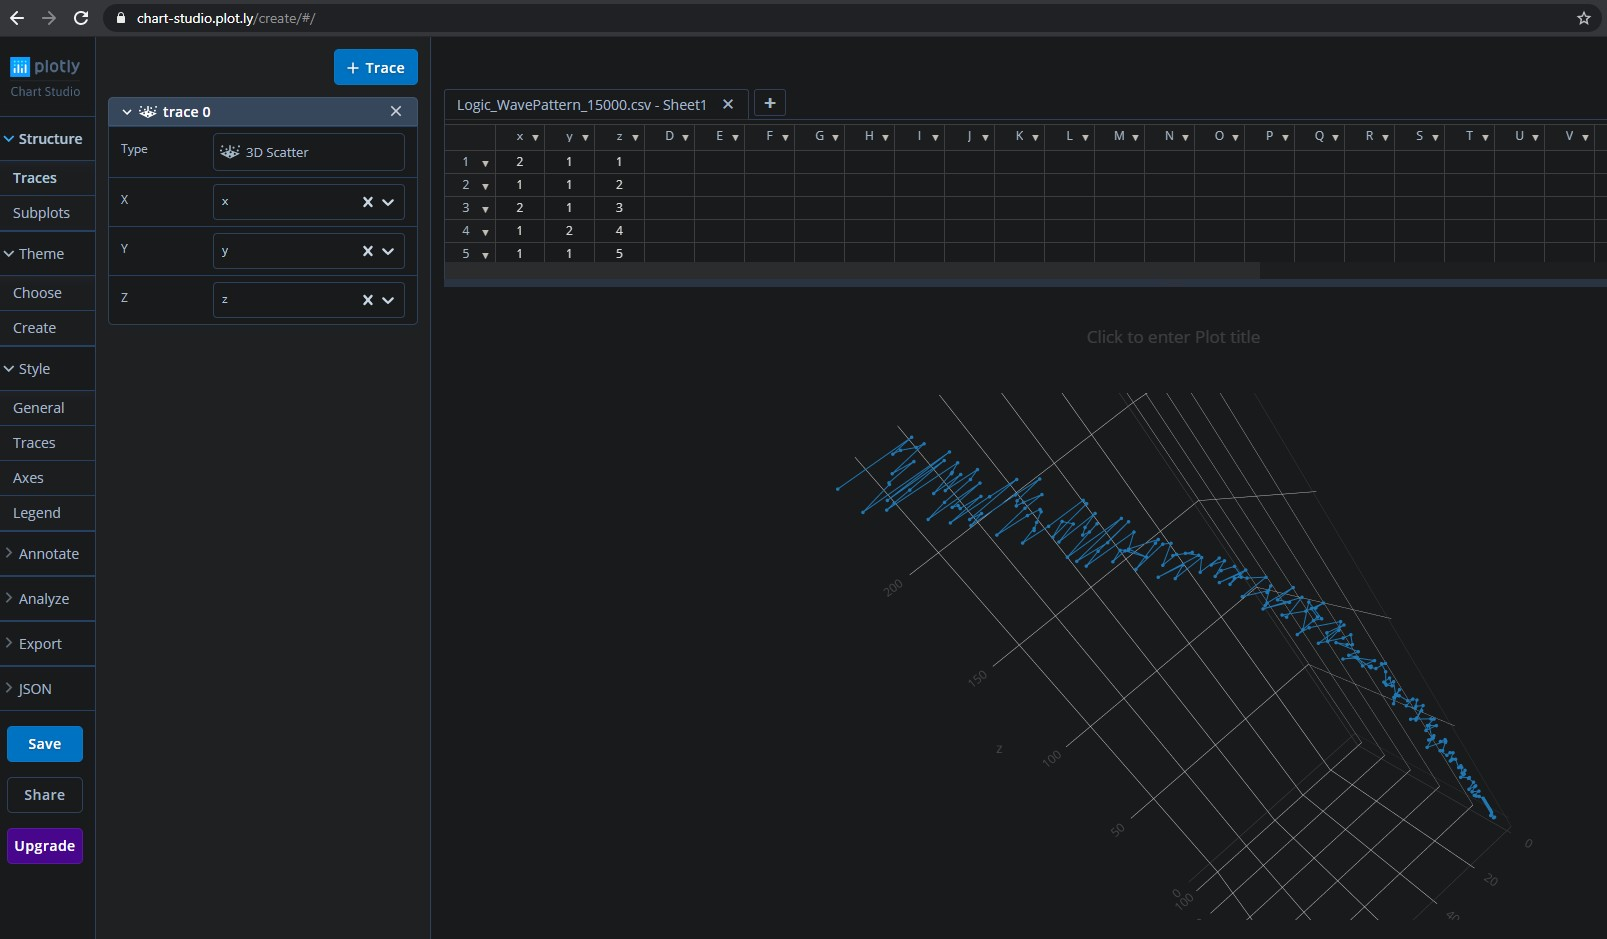
\includegraphics[scale=.35]{sections/images/plotly_3DScatter.jpg}
\floatfoot{O exemplo pode ser acessado em: \url{https://chart-studio.plot.ly/create/?fid=ren.stuchi:5&fid=ren.stuchi:4}.} %\footnotemark.
\end{figure}

\subsection*{BinomialDistribution\_PROB [Code]}
Para execução deste trecho de código é necessário a implementação do BigDecimal, um exemplo dessa implementação, pode ser observado, obedecendo os direitos de licença de software proprietários em \cite{ github_bigdecimal}. Este estudo não distribui e nem se responsabiliza pela porção do código referente à implementação do BigDecimal, ficando essas responsabilidades  à cargo do executor deste trecho de software.

\bigbreak
\begin{lstlisting}
//https://www.mathsisfun.com/data/quincunx-explained.html
void Main()
{
    BinomailDistribuition.Possibilities = 10;
    var results = new List<BigDecimal>();
    results.Load();
    results.Print(true); //send false to print Table 1.
}

public static class BinomailDistribuition
{
    public static int Possibilities = 0;
    static int middleLeft = 0;
    static int middleRight = 0;
    static int resultCount = 0;
    
    public static void Load(this List<BigDecimal> results)
    {
        for (int i = 0; i <= Possibilities; i++)
        {
            var fatorLeft = Fatorial(Possibilities);
            var fatorRight = BigInteger.Multiply(Fatorial(i), Fatorial(Possibilities - i));
            BigInteger fat = BigInteger.Divide(fatorLeft, fatorRight);
            var powLeft = new BigDecimal(1, 0, 1000000000);
            var powRight = new BigDecimal(1, 0, 1000000000);
            if (i != 0)
                powLeft = BigDecimal.Pow(new BigDecimal(5, 1, 1000000000), i);
            if (i != Possibilities)
                powRight = BigDecimal.Pow(new BigDecimal(5, 1, 1000000000), (Possibilities - i));
            var prob = new BigDecimal(fat) * powLeft * powRight;
            results.Add(prob);
        }
    }
    
    public static BigInteger Fatorial(int value)
    {
        BigInteger fatorial = 1;
        for (int n = 1; n <= value; n++)
        {
            fatorial *= n;
        }
        return fatorial;
    }
    
    public static void Print(this List<BigDecimal> results, bool printTableProbability)
    {
        if (!printTableProbability)
        {
            var sum = results.Sum();
            var middle = (middleRight - middleLeft) / 2;
            var middlePercent = ((middleRight - middleLeft) * 14) / 100;
            var list = results.Where((x, i) => i >= middleLeft && i <= middleRight).ToList();
            var listPareto = list.Where((x, i) => i >= (middle - middlePercent) && i <= (middle + middlePercent)).ToList();
            var percentOfSum = (middleRight - middleLeft) * 100 / resultCount;
            var sumPercent = sum * new BigDecimal(100, 0, 1000000000);
            var paretoResult = new BigDecimal(0, 0, 1000000000);
            listPareto.ForEach(x => { paretoResult = paretoResult + x; });

            sumPercent.Dump("sum");
            middleLeft.Dump("middleLeft");
            middleRight.Dump("middleRight");
            (middleRight - middleLeft).Dump("itens of sum");
            percentOfSum.Dump("percent of sum");
            resultCount.Dump("total");
            paretoResult.Dump("20/80");
        }
        else
        {
            results.Dump(); //Valid Binomial distribution    
        }
    }
    
    public static BigDecimal Sum(this List<BigDecimal> results)
    {
        resultCount = results.Count;
        middleLeft = resultCount / 2;
        middleRight = middleLeft * 2 < resultCount ? middleLeft + 1 : middleLeft;

        var sum = middleLeft != middleRight ? results[middleLeft] + results[middleRight] : results[middleRight];
        while ((sum * new BigDecimal(100, 0, 1000000000)) < new BigDecimal(9999, 2, 1000000000))
        {
            middleLeft--;
            middleRight++;
            if (middleLeft >= 0)
                sum = sum + results[middleLeft];
            if (middleRight <= Possibilities)
                sum = sum + results[middleRight];
        }
        return sum;
    }
}

//Exemple of BigDecimal class - https://github.com/dparker1/BigDecimal/blob/
//3e0a4f1ba4c72c0b28d6571fcc6259558be104bd/BigDecimal/BigDecimal.cs
\end{lstlisting}

\bigbreak
\bigbreak
\subsection*{Distribution\_PROB [Code]}
\begin{lstlisting}
//https://exercicios.brasilescola.uol.com.br/exercicios-matematica/
//exercicios-sobre-probabilidade-condicional.htm#questao-1
void Main()
{
    var dice = 2; //Binomial distribution, dice = 2;
    var events = 10;
    var sampling = Math.Pow(dice, events);
    var cartesianProduct = dice.ToArrays(events).CartesianProduct();
    cartesianProduct.PrintGroup(events, dice);
}

public static class CartesianProductContainer
{
    public static IEnumerable<IEnumerable<int>> CartesianProduct(this IEnumerable<IEnumerable<int>> sequences)
    {
        IEnumerable<IEnumerable<int>> emptyProduct = new[] { Enumerable.Empty<int>() };
        var result = sequences.Aggregate(
            emptyProduct,
            (accumulator, sequence) =>
                from accseq in accumulator
                from item in sequence
                select new[] { accseq.Concat(new[] { item }).Sum() });

        return result;
    }

    public static IEnumerable<List<int>> ToArrays(this int dice, int events)
    {
        var result = new List<List<int>>();
        for (int j = 1; j <= events; j++)
        {
            var array = new List<int>();
            for (int i = 1; i <= dice; i++)
                array.Add(i);
            
            result.Add(array);
        }

        return result;
    }
    
    public static void PrintGroup(this IEnumerable<IEnumerable<int>> list, int events, int dice)
    {
        var listCountDict = Enumerable.Range(1, dice * events).ToDictionary(x => x);
        Group(listCountDict, list);
        listCountDict.Dump("Values");
    }

    public static void Group(Dictionary<int, int> dict, IEnumerable<IEnumerable<int>> list)
    {
        foreach (var key in dict.Keys.ToList())
            dict[key] = 0;

        foreach (var item in list)
            dict[item.First()]++;

        var zeroKey = 0;
        foreach (var item in dict)
            if (item.Value == 0) 
                zeroKey = item.Key;
            else continue;

        for (int i = 1; i <= zeroKey; i++)
            dict.Remove(i);
    }
}

\end{lstlisting}


\bigbreak
\subsection*{Logic\_WavePattern [Code]}
\begin{lstlisting}
//http://csharphelper.com/blog/2015/09/draw-a-simple-histogram-in-c/
//https://github.com/naudio/NAudio.WaveFormRenderer
[STAThread]
void Main()
{
  Application.EnableVisualStyles();
  Application.Run(new MainForm());
}

public partial class MainForm : Form
{
  public MainForm()
  {
    InitializeComponent();
  }
  //###########################################################################
  private const int LENGHT = 15000;
  private const int GROUP = 10;
  private bool nestedHistogram = false;
  //###########################################################################
  private double m_dZoomscale = 1.0;
  public static double s_dScrollValue = .05;
  private Point MouseDownLocation;
  private Matrix transform = null;
  private NumbsOfCentralLimitTheorem.HistogramResult histogramResult = null;
  private bool printed = false;

  // Make random histogram data.
  private void MainForm_Load(object sender, EventArgs e)
  {
    histogramResult = GetHistogramOfCentralLimitTheorem(LENGHT, GROUP);

    // Make a transformation to the PictureBox.
    RectangleF data_bounds = new RectangleF(0, 0, histogramResult.Size, histogramResult.MaxValue * 2);
    PointF[] points =
    {
        new PointF(0, pictHistogram.ClientSize.Height),
        new PointF(pictHistogram.ClientSize.Width, pictHistogram.ClientSize.Height),
        new PointF(0, 0)
      };
    transform = new Matrix(data_bounds, points);
  }

  private void pictHistogram_Paint(object sender, PaintEventArgs e)
  {
    DrawHistogram(e.Graphics, pictHistogram.BackColor, histogramResult,
      pictHistogram.ClientSize.Width, pictHistogram.ClientSize.Height);
  }

  private void pictHistogram_Resize(object sender, EventArgs e)
  {
    pictHistogram.Refresh();
  }

  // Draw a histogram.
  private void DrawHistogram(Graphics gr, Color back_color,
    NumbsOfCentralLimitTheorem.HistogramResult histogramResult, int width, int height)
  {
    PrintResult();
    gr.Clear(back_color);
    gr.Transform = transform;
    gr.ScaleTransform((float)m_dZoomscale, (float)m_dZoomscale);
    FillRectangle(gr, Color.Black, histogramResult.Up, histogramResult.MaxValue, false);
    FillRectangle(gr, Color.Gray, histogramResult.Down, histogramResult.MaxValue, true);
  }
  
  private void PrintResult()
  {
    if (!printed)
    {
      printed = true;
      var listTuple = new List<(float x, float y, float z)>();
      float previousValueOfZ = 0;
      for (int i = 0; i < histogramResult.Up.Count(); i++)
      {
        if (histogramResult.Up[i] != 0.0001f && histogramResult.Down[i] != 0.0001f)
        {
          if (histogramResult.Up[i] % 1 == 0)
            previousValueOfZ = (int)(previousValueOfZ + 1f);
          else 
            previousValueOfZ += 0.1f;
          var tuple = (x: histogramResult.Up[i], y: histogramResult.Down[i], z: previousValueOfZ);
          listTuple.Add(tuple);
        }
      }
      Console.WriteLine("x,y,z");
      foreach (var tuple in listTuple)
        Console.WriteLine(tuple.x.ToString() + "," + tuple.y.ToString() + "," + tuple.z.ToString());
    }
  }

  protected void FillRectangle(Graphics gr, Color color, float[] arrayValues, float maxValue, bool down)
  {
    using (Pen thin_pen = new Pen(color, 0))
    {
      for (int i = 0; i < histogramResult.Down.Length; i++)
      {
        RectangleF rect;
        if (!down)
          rect = new RectangleF(i, maxValue, 1, arrayValues[i]);
        else
          rect = new RectangleF(i, maxValue - arrayValues[i], 1, arrayValues[i]);
        using (Brush the_brush = new SolidBrush(color))
        {
          gr.FillRectangle(the_brush, rect);
          gr.DrawRectangle(thin_pen, rect.X, rect.Y, rect.Width, rect.Height);
        }
      }
    }
  }

  protected void pictHistogram_OnMouseWheel(object sender, MouseEventArgs mea)
  {
    pictHistogram.Focus();
    if (pictHistogram.Focused == true && mea.Delta != 0)
      ZoomScroll(mea.Location, mea.Delta > 0);
  }

  private void ZoomScroll(Point location, bool zoomIn)
  {
    transform.Translate(-location.X, -location.Y);
    if (zoomIn)
      m_dZoomscale = m_dZoomscale + s_dScrollValue;
    else
      m_dZoomscale = m_dZoomscale - s_dScrollValue;
    transform.Translate(location.X, location.Y);
    pictHistogram.Invalidate();
  }

  private void pictHistogram_MouseDown(object sender, MouseEventArgs e)
  {
    if (e.Button == System.Windows.Forms.MouseButtons.Left)
      MouseDownLocation = e.Location;
  }

  private void pictHistogram_MouseMove(object sender, MouseEventArgs e)
  {
    if (e.Button == System.Windows.Forms.MouseButtons.Left)
    {
      transform.Translate((e.Location.X - MouseDownLocation.X)
        / 40, (e.Location.Y - MouseDownLocation.Y) / 40, MatrixOrder.Append);
      this.Refresh();
    }
  }

  private NumbsOfCentralLimitTheorem.HistogramResult GetHistogramOfCentralLimitTheorem(int length, int group)
  {
    var numbsOfCentralLimitTheorem = new NumbsOfCentralLimitTheorem();
    numbsOfCentralLimitTheorem.NestedHistogram = nestedHistogram;
    numbsOfCentralLimitTheorem.RandomResult(length);
    return numbsOfCentralLimitTheorem.GenerateHistogram(group);
  }
}

partial class MainForm
{
  private System.ComponentModel.IContainer components = null;

  protected override void Dispose(bool disposing)
  {
    if (disposing && (components != null))
      components.Dispose();
    base.Dispose(disposing);
  }

  private void InitializeComponent()
  {
    this.pictHistogram = new System.Windows.Forms.PictureBox();
    ((System.ComponentModel.ISupportInitialize)(this.pictHistogram)).BeginInit();
    this.SuspendLayout();

    // pictHistogram
    this.pictHistogram.Anchor = ((System.Windows.Forms.AnchorStyles)((((System.Windows.Forms.AnchorStyles.Top
          | System.Windows.Forms.AnchorStyles.Bottom)
          | System.Windows.Forms.AnchorStyles.Left)
          | System.Windows.Forms.AnchorStyles.Right)));
    this.pictHistogram.BackColor = System.Drawing.Color.White;
    this.pictHistogram.Cursor = System.Windows.Forms.Cursors.Cross;
    this.pictHistogram.Location = new System.Drawing.Point(8, 6);
    this.pictHistogram.Name = "pictHistogram";
    this.pictHistogram.Size = new System.Drawing.Size(550, 250);
    this.pictHistogram.TabIndex = 1;
    this.pictHistogram.TabStop = false;
    this.pictHistogram.Resize += new System.EventHandler(this.pictHistogram_Resize);
    this.pictHistogram.Paint += new System.Windows.Forms.PaintEventHandler(this.pictHistogram_Paint);
    this.pictHistogram.MouseWheel += new System.Windows.Forms.MouseEventHandler(this.pictHistogram_OnMouseWheel);
    this.pictHistogram.MouseDown += new System.Windows.Forms.MouseEventHandler(this.pictHistogram_MouseDown);
    this.pictHistogram.MouseMove += new System.Windows.Forms.MouseEventHandler(this.pictHistogram_MouseMove);

    // MainForm
    this.AutoScaleDimensions = new System.Drawing.SizeF(6F, 13F);
    this.AutoScaleMode = System.Windows.Forms.AutoScaleMode.Font;
    this.ClientSize = new System.Drawing.Size(563, 262);
    this.Controls.Add(this.pictHistogram);
    this.Name = "MainForm";
    this.Text = "Logic_WavePattern";
    this.Load += new System.EventHandler(this.MainForm_Load);
    ((System.ComponentModel.ISupportInitialize)(this.pictHistogram)).EndInit();
    this.ResumeLayout(false);
  }

  internal System.Windows.Forms.PictureBox pictHistogram;
}

public class NumbsOfCentralLimitTheorem
{
  public float[] ResultList { get; set; }
  public int ResultLength { get; set; }
  public float[] LastList { get; set; }
  public float[] CurrentList { get; set; }
  public int SizeLastList { get; set; }
  public Dictionary<int, float> Histogram { get; set; }
  public bool NestedHistogram { get; set; }
  private int nestedCountDown = 2;

  public NumbsOfCentralLimitTheorem()
  {
    NestedHistogram = false;
    SizeLastList = 2;
    StartLastList();
    StartCurrentList();
  }

  public float[] RandomResult(int length)
  {
    ResultLength = length;
    ResultList = new float[length];
    Random rnd = new Random();
    for (int x = 0; x < length; x++)
    {
      float lineSum = 0;
      for (int i = 1; i < SizeLastList; i++)
      {
        var lastValueLeft = LastList[i - 1];
        var lastValueRight = LastList[i];
        var rndValue = (float)rnd.NextDouble(lastValueLeft, lastValueRight);
        lineSum = lineSum + (rndValue - lastValueLeft);
        CurrentList[i] = rndValue;
      }
      if (lineSum != 0)
        ResultList[x] = lineSum;
      SizeLastList++;
      LastList = CurrentList;
      StartCurrentList();
    }
    return ResultList;
  }

  public HistogramResult GenerateHistogram(int group)
  {
    Histogram = new Dictionary<int, float>();
    var minValue = ResultList.Min();
    var maxValue = ResultList.Max();
    var rangeValue = maxValue - minValue;
    var amountOfGroups = ResultLength / group;
    var intervalValue = rangeValue / amountOfGroups;
    foreach (var value in ResultList)
    {
      int key = (int)(value / intervalValue);
      if (!Histogram.ContainsKey(key))
        Histogram[key] = 0;
      Histogram[key]++;
    }
    var histogramResult = HistogramResult.Get(Histogram);
    if (NestedHistogram)
      printMaxInterval(histogramResult, Histogram, intervalValue, group);
    return histogramResult;
  }

  public Dictionary<int, float> GenerateHistogram(List<float> ResultList, KeyValuePair<int, float> keyValue, int group)
  {
    Histogram = new Dictionary<int, float>();
    var minValue = ResultList.Min();
    var maxValue = ResultList.Max();
    var rangeValue = maxValue - minValue;
    var amountOfGroups = ResultList.Count / group;
    var intervalValue = rangeValue / amountOfGroups;
    foreach (var value in ResultList)
    {
      int key = (int)(value / intervalValue);
      if (!Histogram.ContainsKey(key))
        Histogram[key] = keyValue.Value;
      Histogram[key]-= (1.0F / group);
    }
    return Histogram;
  }

  private void printMaxInterval(HistogramResult histogramResult, Dictionary<int, float> histogram, float intervalValue, int group)
  {
    var histogramOrdered = histogram.OrderBy(x => x.Key);
    var middle = histogram.Count / 2;
    var valueUp = histogramOrdered.ElementAt(middle - nestedCountDown);
    var valueDown = histogramOrdered.ElementAt(middle + nestedCountDown);
    var listUp = GenerateList(valueUp, intervalValue);
    var listDown = GenerateList(valueDown, intervalValue);
    var histogramUp = GenerateHistogram(listUp, valueUp, group);
    var histogramDown = GenerateHistogram(listDown, valueDown, group);
    listUp = histogramUp.Values.ToList();
    listDown = histogramDown.Values.ToList();
    var listCountMin = listUp.Count > listDown.Count ? listDown.Count : listUp.Count;
    histogramResult.Up = RefreshArray(histogramResult.Up, listUp, listCountMin);
    histogramResult.Down = RefreshArray(histogramResult.Down, listDown, listCountMin);
  }
  
  private float[] RefreshArray(float[] array, List<float> newItens, int listCountMin)
  {
    var newArray = new float[array.Count() + listCountMin];
    var rangeValueListMin = newArray.Count() - nestedCountDown - listCountMin;
    var rangeValueListMax = newArray.Count() - nestedCountDown;
    for (int i = 1; i <= nestedCountDown; i++)
      newArray[newArray.Count() - i] = array[array.Count() - i];
    for (int i = 0; i < newArray.Count() - nestedCountDown; i++)
    {
      if (i >= rangeValueListMin && i <= rangeValueListMax)
        newArray[i] = newItens[i - rangeValueListMin];
      else
        newArray[i] = array[i];
    }
    return (float[])newArray.Clone();
  }

  private List<float> GenerateList(KeyValuePair<int, float> keyValue, float intervalValue)
  {
    var minValueInterval = keyValue.Key * intervalValue;
    var maxValueInterval = minValueInterval + intervalValue;
    var internalList = new List<float>();
    foreach (var value in ResultList)
    {
      if (value >= minValueInterval && value <= maxValueInterval)
        internalList.Add(value);
    }
    return internalList;
  }

  private void StartCurrentList()
  {
    var sizeCurrentList = SizeLastList + 1;
    CurrentList = new float[sizeCurrentList];
    CurrentList[0] = 0;
    CurrentList[sizeCurrentList - 1] = float.MaxValue / 2;
  }

  private void StartLastList()
  {
    LastList = new float[SizeLastList];
    LastList[0] = 0;
    LastList[SizeLastList - 1] = float.MaxValue / 2;
  }

  public class HistogramResult
  {
    public int Size { get; set; }
    public float MaxValue { get; set; }
    public float[] Up { get; set; }
    public float[] Down { get; set; }

    public static HistogramResult Get(Dictionary<int, float> histogram)
    {
      var histogramOrdered = histogram.OrderBy(k => k.Key);
      var result = new HistogramResult();
      var lengthOdd = histogram.Count % 2 > 0;
      var middle = histogram.Count / 2;
      var middleValue = histogramOrdered.ElementAt(middle).Key;
      result.Size = middleValue;
      result.MaxValue = histogram.OrderBy(k => k.Value).Last().Value;
      result.Up = ArrangeArray(new float[middleValue]);
      result.Down = ArrangeArray(new float[middleValue]);
      for (int i = 0; i < middle; i++)
      {
        var keyValue = histogramOrdered.ElementAt(i);
        result.Up[keyValue.Key] = keyValue.Value;
      }
      for (int i = lengthOdd ? middle + 2 : middle + 1; i < histogram.Count; i++)
      {
        var totalValue = middleValue * 2;
        var keyValue = histogramOrdered.ElementAt(i);
        result.Down[totalValue - keyValue.Key] = keyValue.Value;
      }
      return result;
    }

    private static float[] ArrangeArray(float[] array)
    {
      for (int i = 0; i < array.Length; i++)
        array[i] = 0.0001F;
      return array;
    }
  }
}

public static class rndExtension
{
  public static double NextDouble(this Random rng, double minimum, double maximum)
  {
    return rng.NextDouble() * (maximum - minimum) + minimum;
  }
}
\end{lstlisting}

\end{apendicesenv}